\section{Proof of concept}\label{sec:proof-of-concept}
This section covers an example implementation on how to implement the most prevention techniques mentioned in section \ref{subsec:prevention}. The implementation covers the following prevention techniques which were already explained in the subsection \ref{subsec:prevention}:

\bigskip
\begin{itemize}
    \item TLS (\ref{subsubsec:encrypted-transport-channels})
    \item Certificate pining (\ref{subsubsec:certificate-pinning})
    \item mTLS (\ref{subsubsec:mutal-tls})
    \item Code/Image signing (\ref{subsubsec:code-image-signing})
    \item Versioning (\ref{subsubsec:versioning})
    \item Rollback mechanism (\ref{subsubsec:rollback-mechanism})
\end{itemize}
\bigskip

Flash encryption (\ref{subsubsec:flash-encryption}) and Hardware Security Modules (\ref{subsubsec:hsm}) are not covered due to hardware restrictions of the used ESP32. Flash encryption was dropped due to the possibility of bricking the device in an early development state. Flash encryption can be enabled later with the ESP-IDF configuration menu.

\bigskip
This example implements the above prevention techniques on a ESP32. The ESP32 will securely download a newer version of its own firmware to replace the old one during reboot. The new firmware is served by an update server. The update server is a compilation of various AWS services and is thus hosted in the public cloud of Amazon Web Services (AWS). Figure \ref{fig:poc-architecture} shows the overall system architecture consisting of the device (the ESP32) and the used AWS services. The "Implementation" subsection \ref{subsec:implementation} explains more about each AWS service and its respective use case.

\bigskip
\begin{figure}[H]
    \centering
    %\includesvg[width=0.8\textwidth]{proof-of-concept/assets/architecture.drawio.svg}
    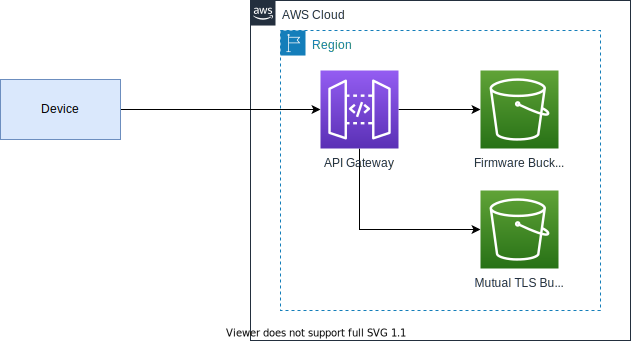
\includegraphics[width=0.8\textwidth]{proof-of-concept/assets/architecture.drawio.png}
    \caption{Basic system architecture}\label{fig:poc-architecture}
\end{figure}

\newpage
\subsection{Requirements}
The following hardware, tools and more is required to run this proof of concept.

\paragraph{Python:} Python 3.8 and above is recommended.

\paragraph{AWS Account:} This example uses AWS to represent the update server. Different AWS services provide the necessary server side protections. A preconfigured aws-cli\footnote{\url{https://docs.aws.amazon.com/cli/latest/userguide/install-cliv2.html}} is required to set up the infrastructure automatically with the code provided inside the GitHub repository.

\paragraph{Terraform:} Serves as infrastructure as code tool \cite{HashiCorp}. For this example, the developer can automatically set up the required infrastructure at AWS by using the provided terraform files inside the repository. Requires aws-cli!

\paragraph{OpenSSL:} Used to generate certificates and more. Other tools for certificate generation are also applicable.

\paragraph{ESP32:} This example shows how an OTA update process can be implemented on a ESP32. The testing environment for this paper was driven by a ESP32 Dev Kit C V4 NodeMCU but the most ESP32 boards may be compatible. Even different CPU architectures like the ESP32 C3 which uses \textbf{RISC-V} should be compatible.

\paragraph{ESP-IDF:} Espressif IoT Development Framework is the official framework, by Espressif, for ESP32 development.

\paragraph{ESP-IDF VS Code extension (optional):} This extension\footnote{\url{https://marketplace.visualstudio.com/items?itemName=espressif.esp-idf-extension}} for Visual Studio Code simplifies processes with the ESP-IDF like installing, building the project, flashing and attaching to the serial monitor. This extension is not required, but can speed up the entire development process.

\subsection{Implementation}\label{subsec:implementation}

\textit{
Before proceeding, note it is strongly recommended to \textbf{not} use the shown example code in any production grade environments. If you plan to do so, keep in mind this example isn't battle tested and may also contain security flaws. \textbf{Use at your own risk!}}

\vspace{\baselineskip}
The code for this example implementation can be found on my GitHub repository\footnote{\url{https://github.com/lukaskirner/ota-security}} under the folder path "\textit{./demo}". For more, detailed instructions and specific tool requirements, follow the README files inside the mentioned repository. This section gives a brief overview about the implementation. This section does not cover every specific detail!

%%%%%%%%%%%%%% Cloud
\subsubsection{Update Server}
The update server must also implement and provide certain things to ensure a secure update process. This example serves the new firmware for the device inside an AWS Simple Storage Service (S3 bucket) as already shown in figure \ref{fig:poc-architecture}. Furthermore the storage service isn't accessible by the public. To get access to the new firmware file, the device connects to an AWS API Gateway which handles the access to the S3 bucket. The API Gateway is the only service which can access the previously mentioned S3 bucket. In addition to handling the access to the firmware file, the gateway also handles the transport encryption with TLS and the authentication via mutual TLS (mTLS). To make the mutual TLS at the API gateway work, the developer needs to provide certificates inside a dedicated S3 bucket. The tool \textbf{OpenSSL} can be used to generate these certificates. The following listing \ref{lst:openssl} shows the generation of the necessary certificates with OpenSSL.

\vspace{10pt}
\begin{lstlisting}[caption={Generating certificates wiht OpenSSL},label={lst:openssl},captionpos=b,frame=single]
openssl genrsa -out my_client.key 2048
openssl req -new -x509 -days 3650 \
    -key my_client.key \
    -out my_client.pem
\end{lstlisting}

\textit{The whole cloud structure can be established by using terraform and the corresponding files (`./demo/terraform`) stored inside the GitHub repository.}

%%%%%%%%%%%%%% Device
\subsubsection{Device}
The device implements the most parts of the secure update process. Figure \ref{fig:poc-activity-diagram} shows a general overview of the activities made in operational state. The abbreviation FW in figure \ref{fig:poc-activity-diagram} stands for firmware. After the entry point the bootloader boots the system with the newest firmware in the flash. The bootloader checks if the new firmware is signed correctly. The verification of the signature is checked with the secure boot key. The key is provided by the older firmware or by the factory firmware if no older firmware exists. After a successful boot, the app starts. The app contains the code for the device to do what the device is supposed to do. For the OTA update an additional task is included. This "update" task handles all the firmware update related tasks. For example, the task connects to the update server to check if new firmware is available. During the connection, the server certificate is also checked and the device authenticates itself via mTLS. If new firmware is available to download this task will do so. The successful download will then trigger the reboot to apply the new firmware. The reboot can also be triggered by a press of the "Reset" button on the ESP32 dev board.

\begin{figure}[H]
    \centering
    \fontsize{8}{10}\selectfont
    %\includesvg[width=\textwidth]{proof-of-concept/assets/activity-diagram.drawio.svg}
    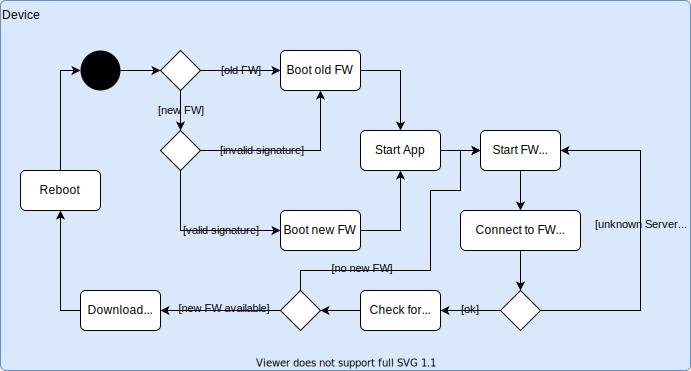
\includegraphics[width=\textwidth]{proof-of-concept/assets/activity-diagram.drawio.png}
    \caption{Device OTA update activity diagram}\label{fig:poc-activity-diagram}
\end{figure}

For the implementation of the update task ESP-IDF provides helpful libraries. There is a library to do OTA firmware updates. This library implements the task of downloading the firmware to the correct partition. Security features must be added by the developer. For example by adding an HTTP client, like the one shown in listing \ref{lst:esp_http_client_config_t}, which supports certificate pinning and mTLS. The necessary certificates mTLS and server cert check must be embedded as text files during the firmware build. The developer is also required to implement the firmware version check.

\vspace{\baselineskip}
\begin{lstlisting}[caption={HTTP client},label={lst:esp_http_client_config_t},captionpos=b,frame=single]
esp_http_client_config_t config = {
    .url = "https://your-update-server.com",
    .cert_pem = (char *) server_cert_pem_start,
    .client_key_pem = (char *) client_cert_key_start,
    .client_cert_pem = (char *) client_cert_pem_start
};
\end{lstlisting}

To be able to download new firmware a partition table must be provided because the default one does not support OTA updates. The default ESP-IDF project only has one app partition which isn't enough. To be able to download updates and apply them later, additional partitions must be added. ESP-IDF comes with a pre-written partition table for OTA updates. The pre-written table is called "Factory app, two OTA definitions" and can be chosen in the ESP-IDF configuration menu. This partition table includes one factory partition, where the initial code is located, and two OTA partitions where newer versions get stored by the OTA update library. It should be noted the flash size must be increased also to at least match the sum of all partitions of the partition table.

\bigskip
To check the signature validity of the selected firmware, ESP-IDF provides a simple check box in the configuration menu. To check the signing during the boot procedure the option "Bootloader verifies app signatures" must be enabled. Without this option enabled, signing images has no effect. The validity check requires the developer to provide a signing key which can be generated with the `espsecure.py` program. To automatically perform the signing process during the build, the option "Sign binaries during build" can be enabled too. 

%%%%%%%%%%%%%% Run
\subsubsection{Run}
After flashing the factory firmware to the ESP32 the device starts at the entry point of figure \ref{fig:poc-activity-diagram}. At this moment there is no new firmware available in the S3 bucket. To provide new firmware the developer is required to clean the build folder of the firmware project and rebuild it with a new version. The version string can be incremented in the `version.txt` file. After a successful build, the firmware needs to be uploaded into the corresponding S3 bucket. By resetting the device, pressing the reset button, a reboot is triggered. The device starts again at the entry point of figure \ref{fig:poc-activity-diagram}. This time new firmware is available and will be downloaded and applied. To check if the new firmware was successfully applied, the serial monitor logs the currently running firmware version after a successful boot. This version string should now match the version string in `version.txt`

\bigskip
\textit{The provided GitHub repository provides all the necessary code and scripts to test this example on your own. The README file in the repository root directory contains a four-step guide to get this example up and running.}

